\label{chap4}

%TODO: intro to this chapter


% You may title this section "Methods" or "Models". 
% "Models" is not a valid title for PLoS ONE authors. However, PLoS ONE
% authors may use "Analysis" 
%\section*{Materials and Methods}
%\section{Methods}


% Results and Discussion can be combined.
\section{NER Lexicon-based approach}

Let's check the number of terms found by document.

\begin{table}[ht]
    \centering
    \begin{tabular}{lrrr}
    \toprule
    \textbf{Translation}   &   \textbf{Direct Match} &   \textbf{All Match} &   \textbf{Best Match} \\
    \midrule
     \textbf{Human}         &         119.55 &      177.92 &       145.0 \\

     \textbf{Yandex}        &         116.06 &      173.92 &       145.16 \\

     \textbf{Google}        &         120.8 &      179.49 &       147.61 \\

     \textbf{Unbabel}       &         120.92 &      178.86 &       148.16 \\

    \bottomrule
    \end{tabular} 
    \caption{Number of RadLex terms found by document}
    \label{table:terms_by_document}
\end{table}

One of the highlights here is that the All Match approach consistently found more terms than the Best Match approach, which itself found more terms than the Direct Match approach. This makes sense since the All Match approach its the most liberal one in what it considers to be a mention of a RadLex term. The Best Match approach is more conservative than the All Match approach but less than the Direct Match approach, considering lexical variations and word reordering, for example. But in all cases we can see that a lot of terms are being extracted from each document, which gives more significance to the results presented next. 


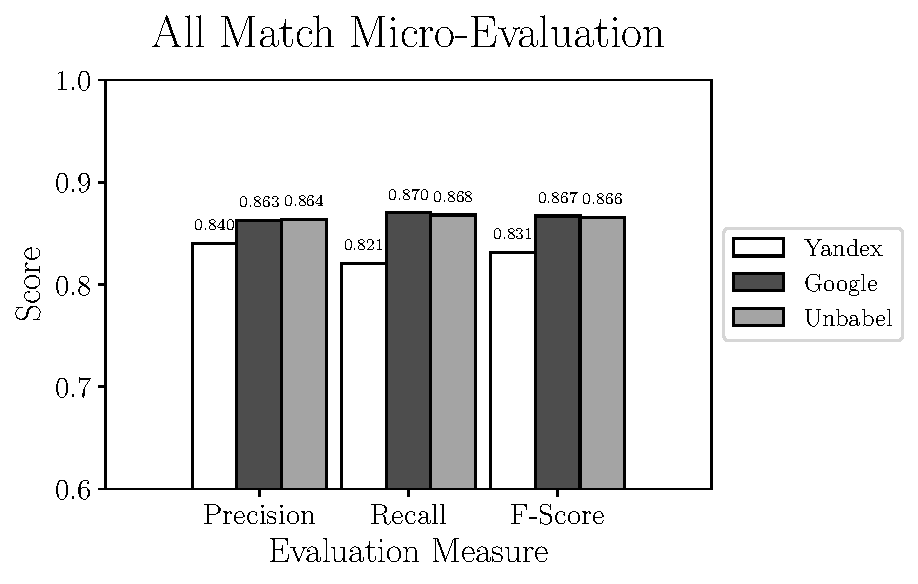
\includegraphics{SupportFiles/plots/all_match_micro_total_plot.pdf}

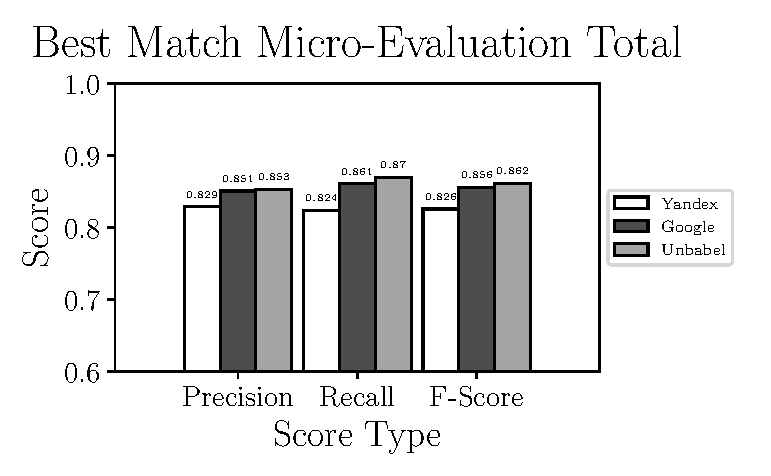
\includegraphics{SupportFiles/plots/best_match_micro_total_plot.pdf}

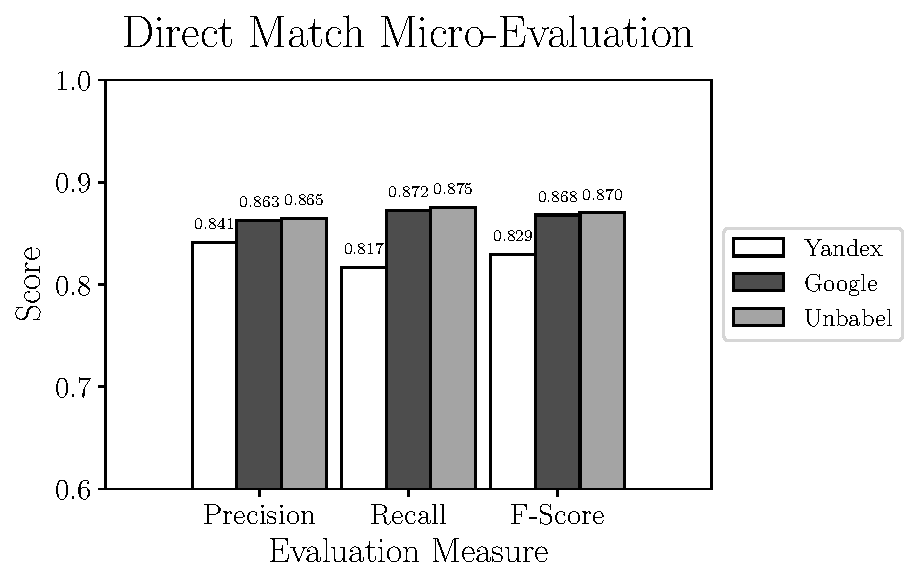
\includegraphics{SupportFiles/plots/direct_match_micro_total_plot.pdf}


The terms extracted from Google translations are more similar to the ones extracted from HT translations than the ones from Yandex translations. This could be just because the human translators used Google Translator to help them in their translation process. This argument loses strength is we assume Google Translate translation outputs changed since the articles were human translated (publication years of the articles used range from 2003 to 2013), but I could not found  data on this. 

The terms extracted from Unbabel and Google translations are really similar, the F-Scores being almost equal. That the translations are similar is not too surprising since the Post-Editing phase at Unbabel is done after MT translation using Google. What could be surprising is that Unbabel does not have a higher score. One conclusion to take from this is that post-editing step on the MT+PE is not useful for this task. 

In the Introduction to the thesis I've proposed the following hypothesis:

\begin{description}
	\item[Hypothesis:] MT+PE is a good trade-off between quality and cost, compared with MT and HT, for translating Radiology reports for the purpose of identifying RadLex terms. 
\end{description}

I've written that for this to be true, "MT+PE quality for the task at hand has to be better than MT quality, enough to compensate its higher cost". This does not hold. For this task, if someone had to choose between Google and Unbabel, this someone would be better off using Google since it is cheaper. 

I've also written that for the hypothesis to be true, "MT+PE quality for the task at hand has to be close enough to HT quality". We've already saw that for this specific task, using MT+PE is not worth it. But the question remains, is it worth to use Google MT? The terms extracted from the Google translations are more similar to the ones from HT translation than Yandex, but they are not extremely similar. If this matters probably depends on the practical application the results of this task would have. 

I will now focus on the "Clinical Finding" and "Anatomical Entity" subtrees of RadLex. These are two of the subtrees that probably would be more important when applying RadLex to a Information Retrieval system. 

\subsection{Clinical Finding and Anatomical Entity Subtrees}

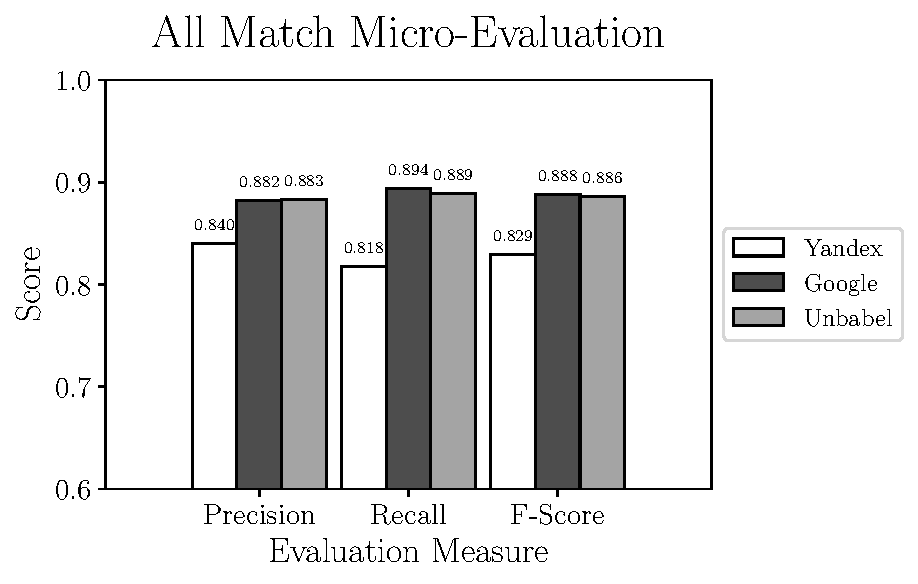
\includegraphics{SupportFiles/plots/all_match_micro_clinical_anatomical_subtrees_plot.pdf}

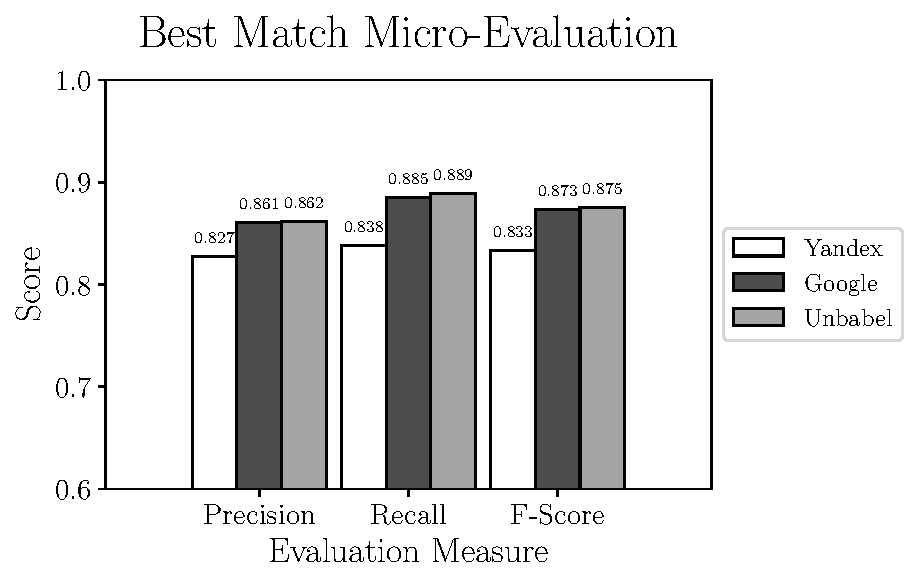
\includegraphics{SupportFiles/plots/best_match_micro_clinical_anatomical_subtrees_plot.pdf}

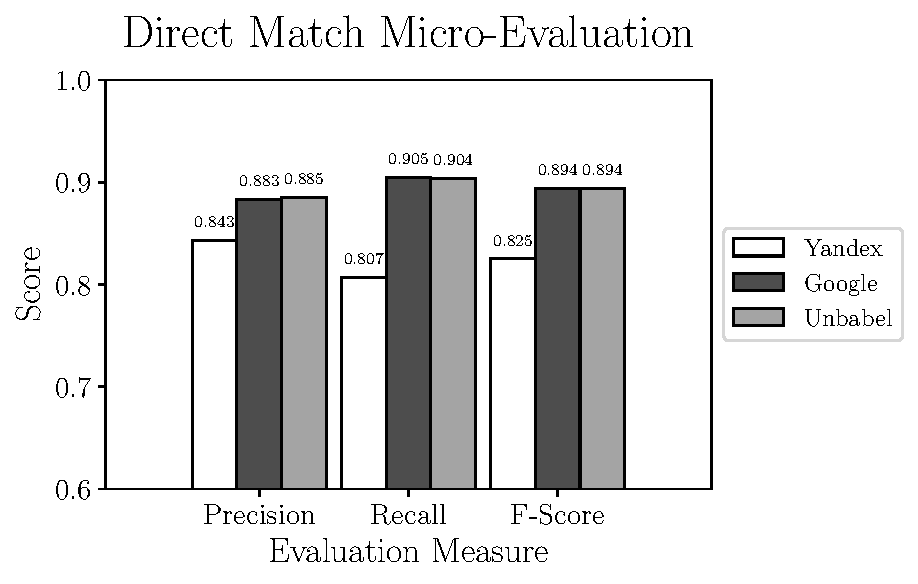
\includegraphics{SupportFiles/plots/direct_match_micro_clinical_anatomical_subtrees_plot.pdf}

Depending on the type of annotation approach and translation it was found between 35.25 and 55.55 "clinical finding" or "anatomical entity" terms per document. The scores obtained are similar to the ones obtained for all terms, with Yandex translation extracted terms being the less similar to the HT translation extracted terms and Google and Unbabel having similar scores. But why these scores? Why do the terms extracted from the MT and MT+PE translated texts are not more similar to the ones extracted from the HT translated texts?

\subsubsection{Error Analysis}

In an attempt to better understand the results, an analysis of the False Positives and False Negatives errors committed by the MT and MT+PE translations, focusing on the terms belonging to the "clinical finding" or "anatomical entity" RadLex subtrees. From preliminary analysis it was known that some of the FPs and FNs are not caused by a bad translation but for other causes, for example, a different translation which is correct but causes a different annotation, e.g., translating "carótida" to "carotid artery" instead of to "carotid" (in the latter translation no term is extracted, in the previous one term is extracted). Still, we expected a higher number of real errors in the Yandex translations compared with the Unbabel or Google translations, since both these type of translation had better scores.

An analysis was done on the FPs and FNs errors committed by Yandex, Google and Unbabel translations in 9 random documents and each error was classified by type. The results from the Best Match Approach were used. As predicted, the percentage of errors by Yandex due to a wrong translation (25\% of 100 FPs or FNs) was higher than the percentage of errors by Google and Unbabel (22\% of 86 and 21\% of 85 FPs or FNs, correspondingly), but only slightly. The reasons for the others FPs and FNs included cases of different translation which is correct but causes a different annotation, as described in the last paragraph and cases in which the word extracted does not have the same meaning in the text as it has in RadLex. For example, the case of extracting the anatomical term "hand" from "(...) on the other hand, it has to be considered that (...)" , in which the word "hand" is used metaphorically. This happens because a ruled-based approach is being used, which does not consider the context of the term. 

Next it was analysed what kind of translation errors were done when the FPs and FNs were caused by real translation errors. These subcategories inlcuded cases in which there was an extra word in the translation, cases in which there was a missing word in the translation, cases when a wrong hyphenization was used, cases in which an acronym was not translated,  cases in which the test translation used a term that was too general, cases in which a wrong lexical variation was used  and cases in which the most correct medical term was not used. Each of these cases had a low number of ocurrings and so it is not worth a deeper analysis. One interesting thing to note is that in the Yandex translations there were some cases (6) in which the original Portuguese word was not even translated. This never happened in the Google and Unbabel translations that were analyzed. This could be explained by the fact that probably Yandex focuses on different languages than Google and so their Portuguese-English translation and/or language models are not so well trained. Most of the errors correspond to just to a general wrong  choice of terms to use as a translation. For example, translate "média" to "middle" instead of "mean" or "lesões de via biliar" to "lesions via bile" instead of "lesions to the biliary tract". This type of problems could probably be solved by training the models used by Google and Yandex with more data, specifically data related to medicine.

One could expect that Unbabel translations would have a lot less mistakes than Google's but this is not always the case. There are situations where errors are even added during the post-editing step. A review of the errors makes us propose that this could be due to the non-medical knowledge of Unbabel editors. For example, a "stroke" is something that occurs in the brain but in one case it was used as something that happens in the heart - someone with some knowledge on medicine would not make this error.


\section{Discussion}





\section{Conclusions}




  
